\documentclass[11pt]{article}

\usepackage{amsmath, amssymb, amsthm}
\usepackage[all]{xy}
\usepackage{color}
\usepackage[pdftex]{graphicx}

\usepackage{rotating}
\usepackage{fullpage}
%\usepackage[top=1.5in,bottom=1.5in,left=2in,right=2in]{geometry}

\begin{document}

\title{H2O IQ - Business Plan}
\author{Mark Fuge \and Shiry Ginosar \and Valkyrie Savage}

\maketitle

\section{Mission Statement}

H2O IQ allows gardeners to water their plants efficiently and consistently whether they are at home or on vacation, available or busy. The system allows gardeners to monitor the moisture intake of their plants, and set a drip irrigation system to automatically achieve the ideal conditions for each plant without over watering or losing water to evaporation. Thus, H2O IQ saves time, conserves water and prevents the guesswork involved with achieving perfect growing conditions.

\section{Price}

Based on existing products targeting the same market share, we project that H2O IQ designed for 2 plant groups will cost \$99 at initial retailers.  We are planning to sell ``kits'' consisting of 2 stakes and a central server for this \$99 price and ``expansion packs'' of single stakes for \$20.

\section{Cost}

The H2O IQ system in year one will cost \$20 for the server/monitoring component and \$4.47 for each in-garden device.  By year five, we expect it to fall to \$16 for the server and \$3.27 for each in-garden device.

\section{H2O IQ System Description}

H2O IQ is a system designed to monitor and actuate drip irrigation in a garden setting. It comprises of in-garden solar powered interactive wireless sensor/actuator devices, an in-garden wireless central server and an online interface. Gardeners can use H2O IQ in one of two modes. In a manual mode, gardeners water their garden themselves and only use the online interface in order to monitor the current moisture level of the plants in order to decide when to water next and how much. In this mode, gardeners can issue a one-time watering command from the online interface in case they are too busy to water on a specific day. In an automatic mode, gardeners set thresholds for an automatic watering regime that will water their plants each time the moisture level gets below the threshold.

Each interactive sensor device is designed to monitor a group of plants of the same species (for instance, one device could monitor a group of tomato plants). The pointy end of the device is intended to be placed in the ground next to one of the plants to be monitored. It consists of a solar-powered moisture sensor, drip irrigation valve actuator, and input buttons. Figure~\ref{fig:plant_vertical} displays the interactive device placed in a potted plant for illustration.

\begin{figure}[h]
\begin{center}
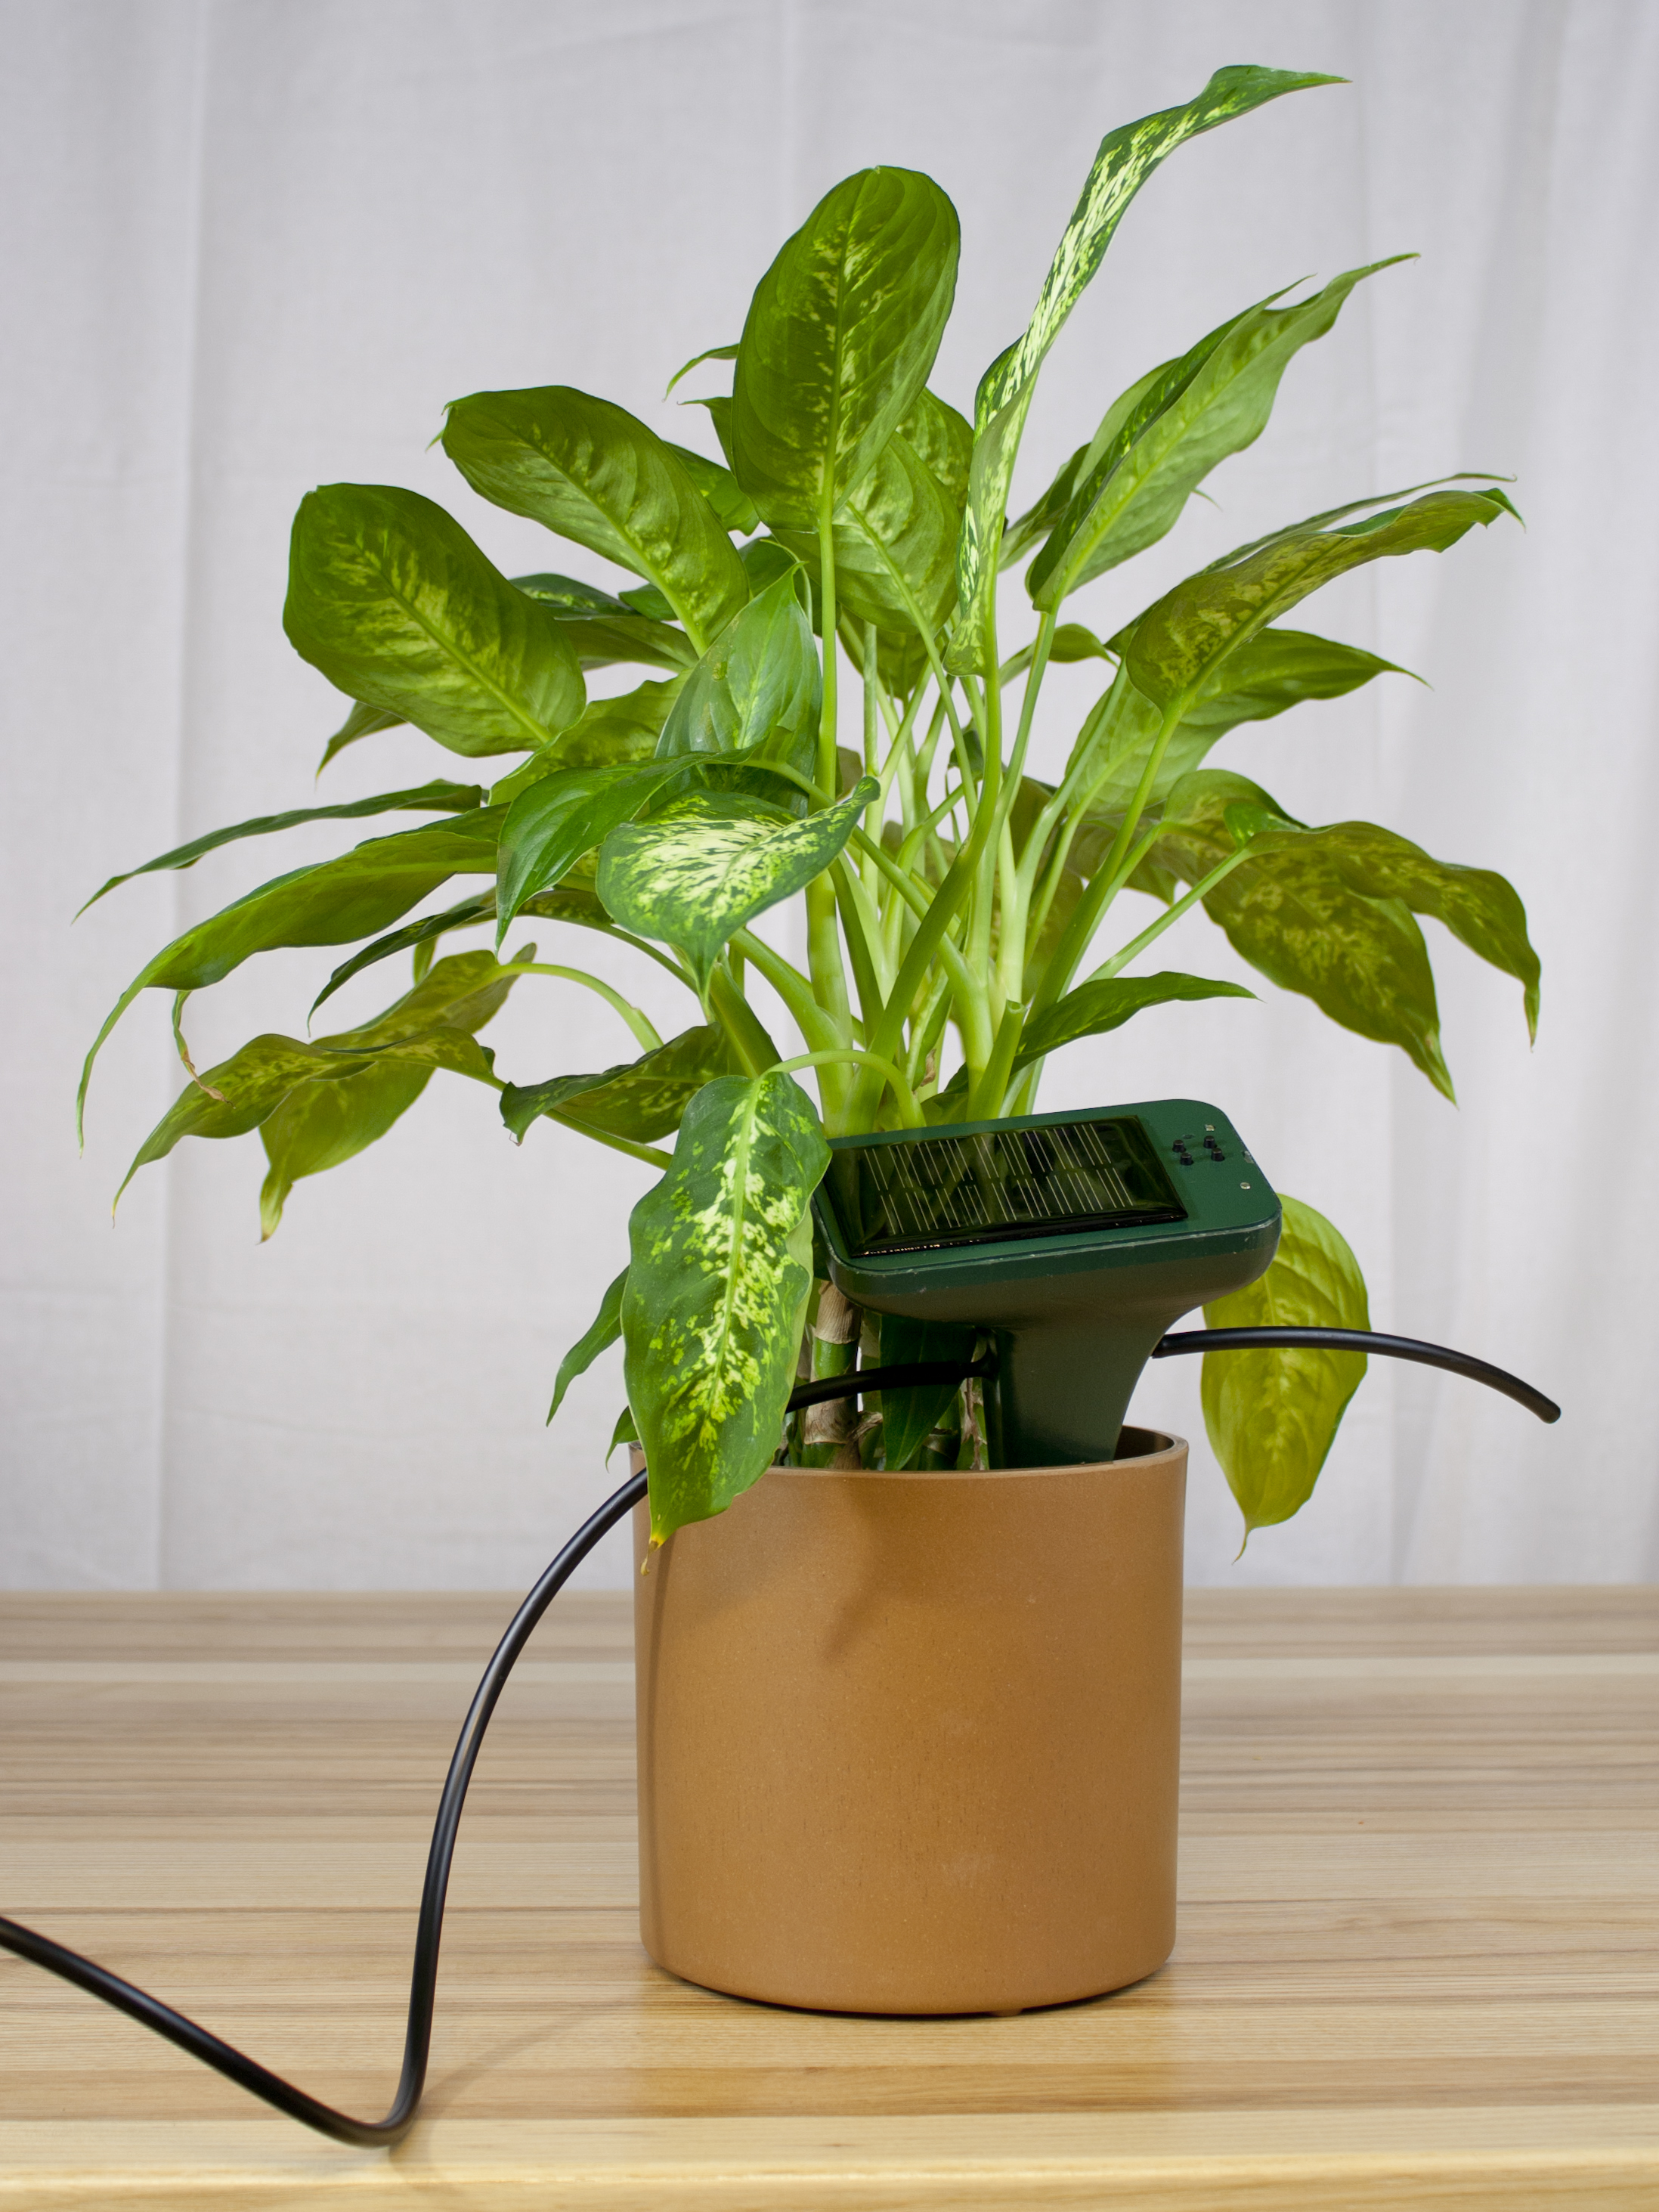
\includegraphics[scale=0.15]{./pngs/plant_vertical.jpg}
\end{center}
\caption{The interactive sensor device placed in a potted plant.}
\label{fig:plant_vertical}
\end{figure}

The central in-garden server is a wireless server designed to control all sensor/actuator devices in one garden. This design reduces the cost of the wireless communication to each sensor, as a lower powered radio connection can be used within the garden. The server also acts as a web server that hosts the online interface.

\subsection{System Architecture}

Figure~\ref{fig:architecture} displays the system architecture.

\begin{figure}[h]
\begin{center}
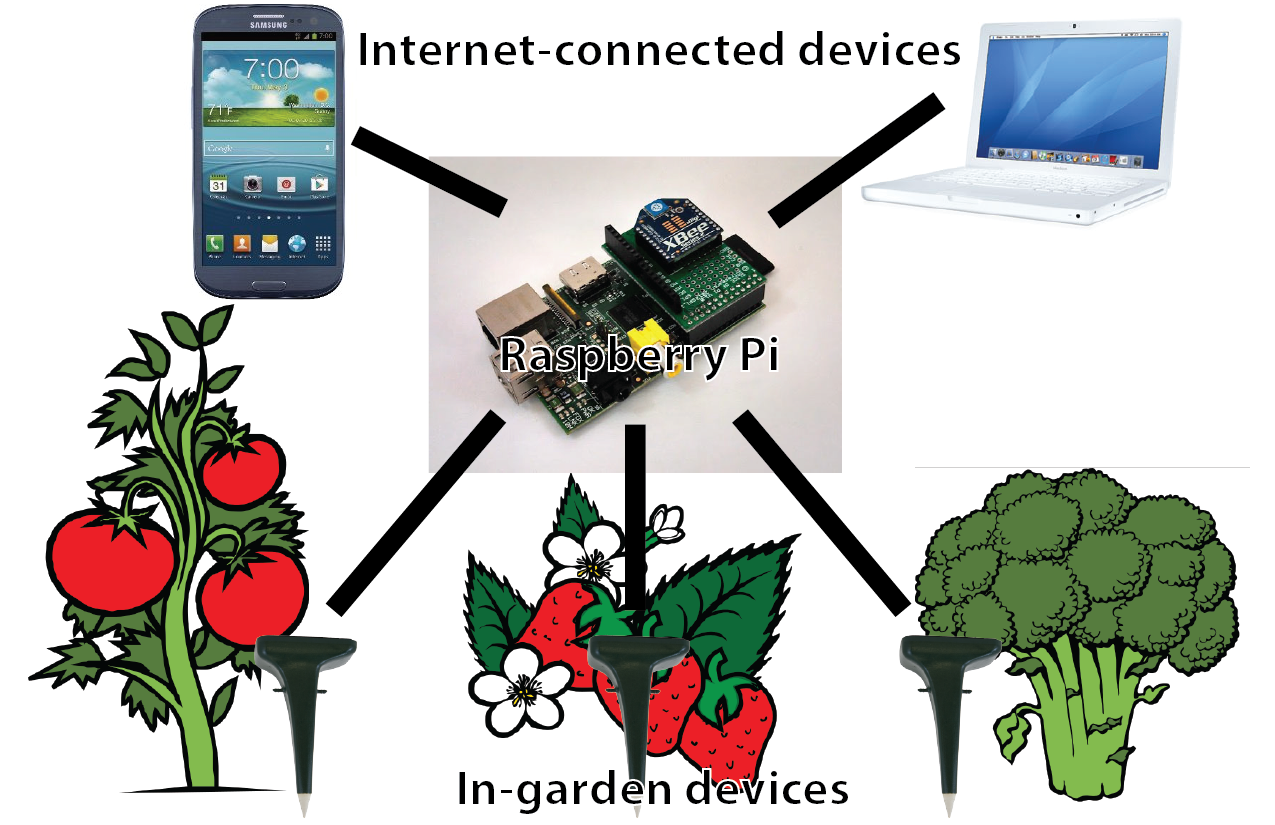
\includegraphics[scale=0.7]{./pngs/architecture.png}
\end{center}
\caption{System architecture.}
\label{fig:architecture}
\end{figure}

The H2O IQ system is built from two principal hardware components: a stake for the garden and a server that is hosted by a Raspberry Pi. Figure~\ref{fig:device} displays the two components side by side.

\begin{figure}[h]
\begin{center}
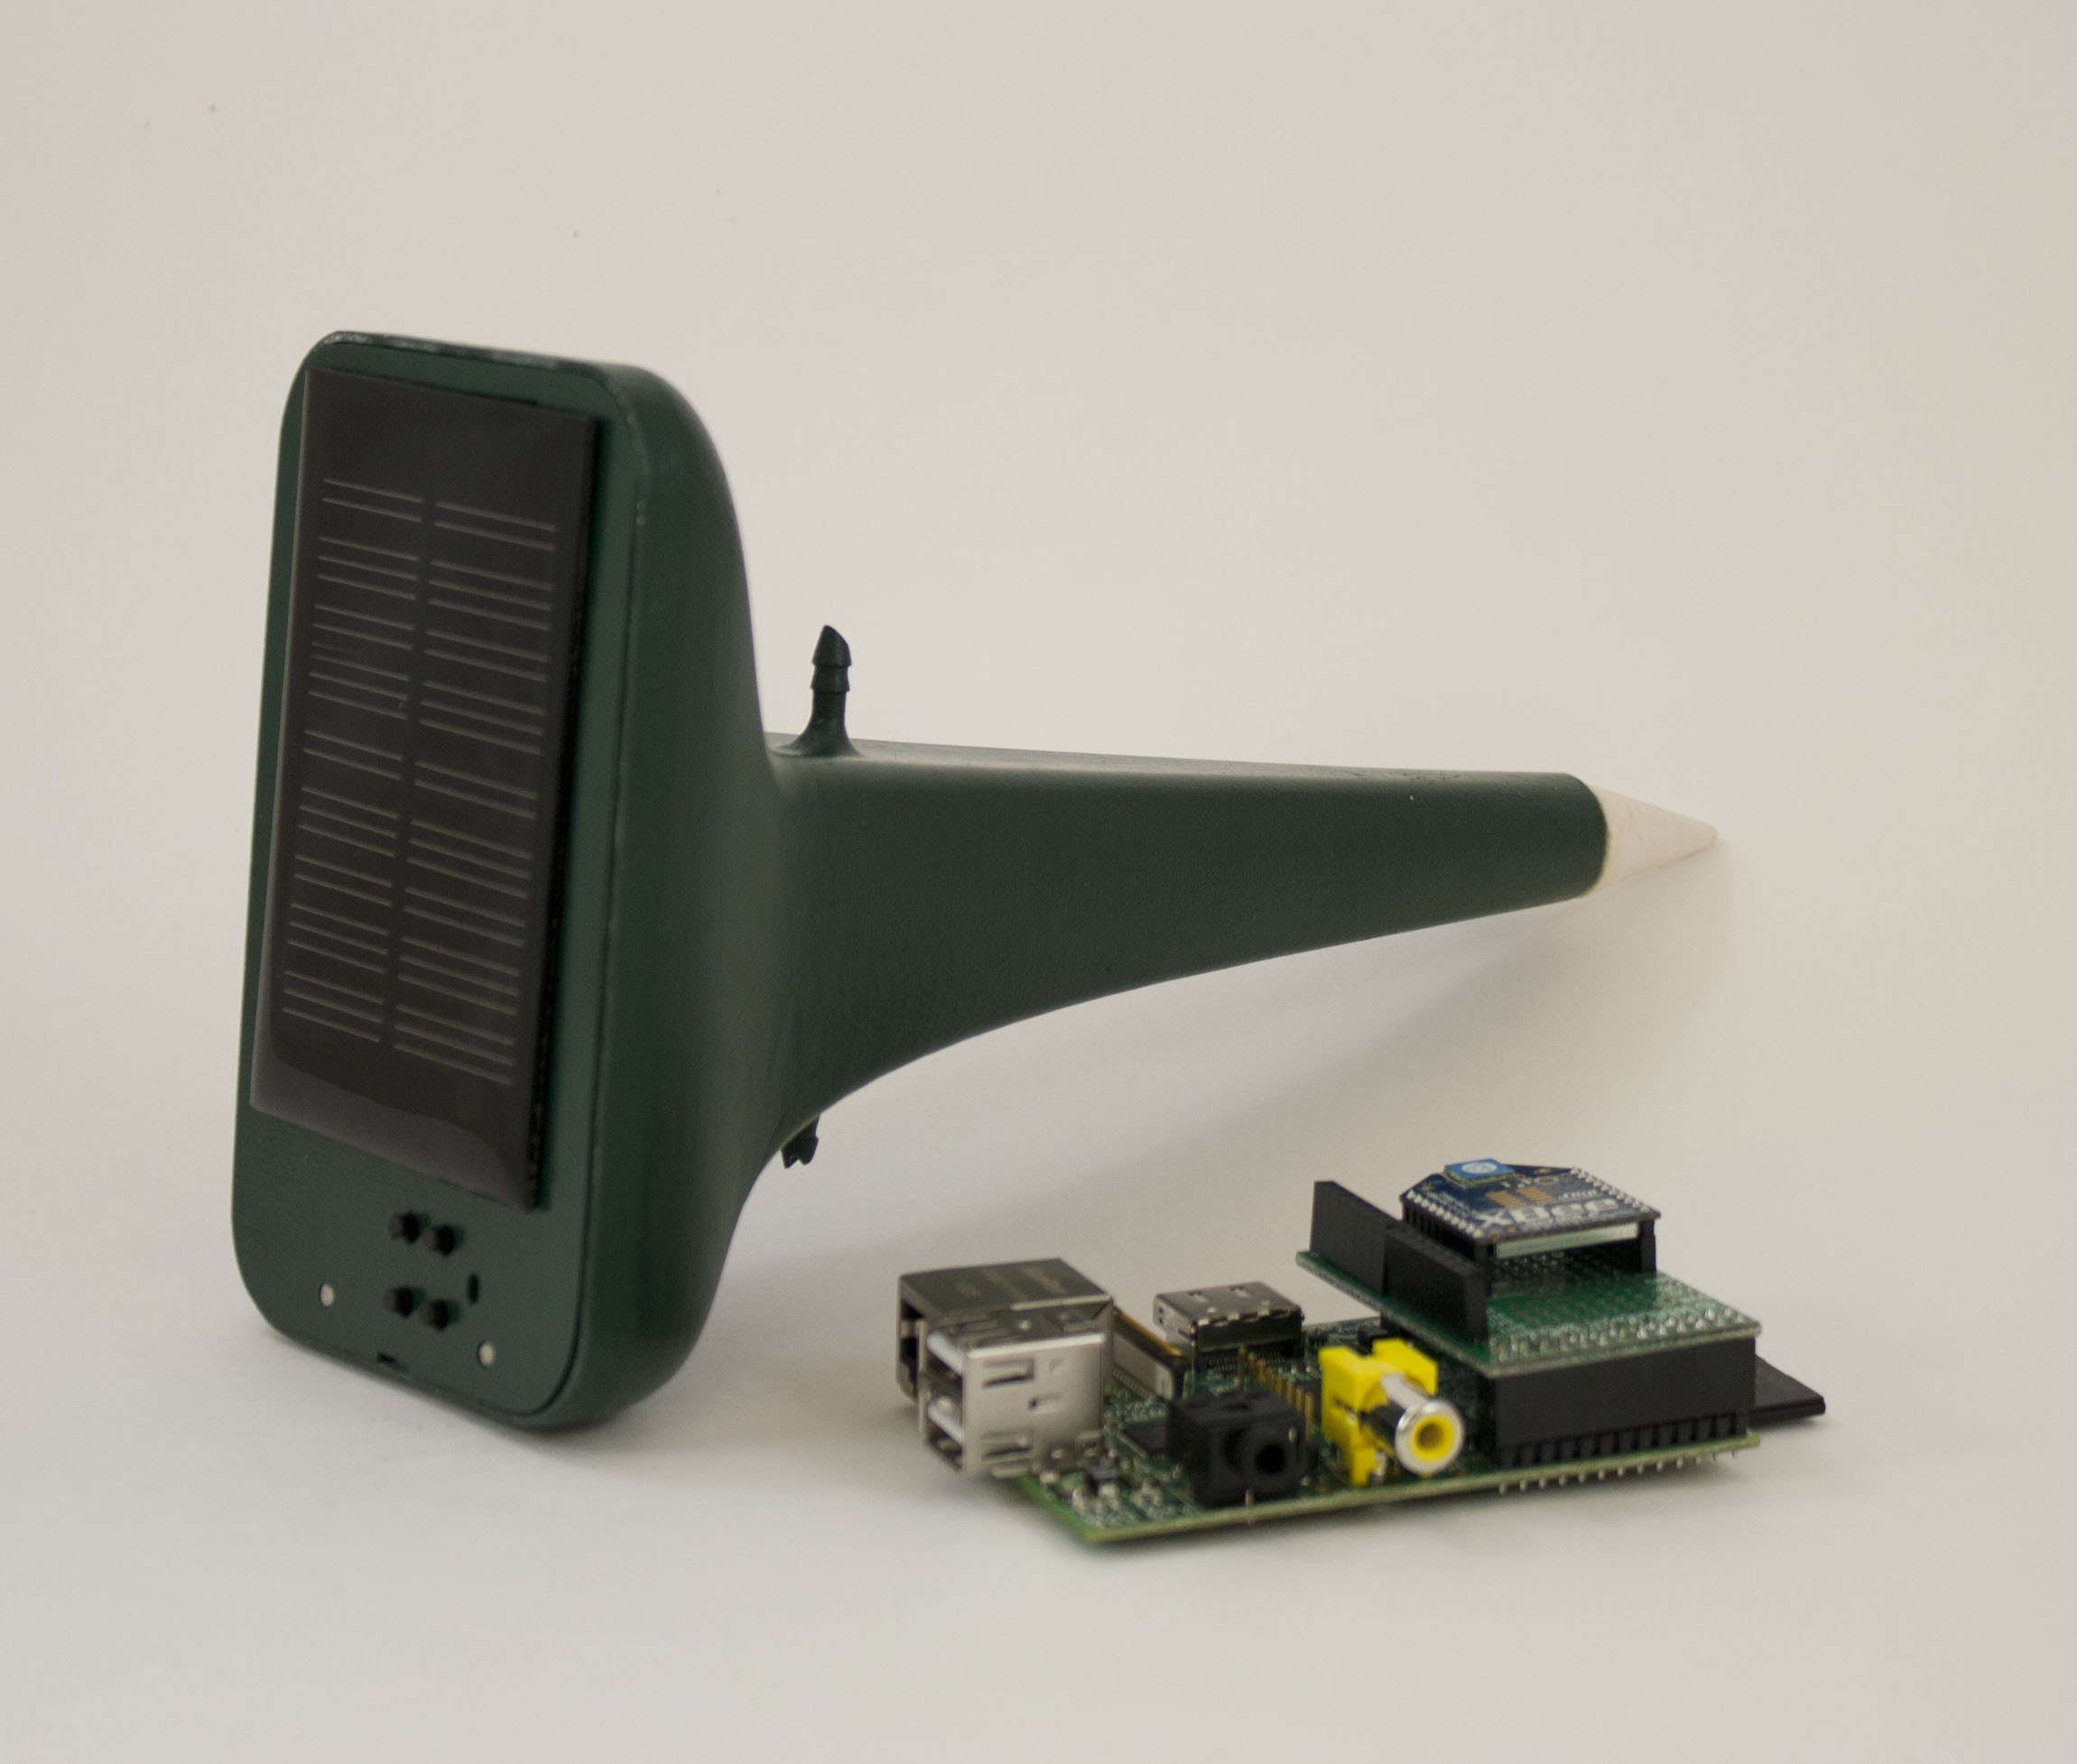
\includegraphics[scale=0.15]{./pngs/device.jpg}
\end{center}
\caption{The main components of the system: a stake for the garden and a Raspberry Pi that hosts the server.}
\label{fig:device}
\end{figure}

The embedded code for the garden stake wakes up once every hour to take a moisture reading and transmit it to the central server via XBee.  The XBee then receives a response containing moisture preference changes that users have input via the web interface.  Putting the device to sleep between these transfers is necessary for power conservation: the LiPo battery that powers the stake can only hold enough charge to make communication viable approximately 15 times without recharging.

The central server has two long-running processes.  One is a continually-running communication loop for receiving communication from the garden stake array: this process takes moisture readings and writes them to a file, then sends a message to the other long-running process that fresh data is available for a particular plant.  The second long-running process is a web server, available for WebSocket-based connections with clients.  Clients can send instructions regarding different moisture goals, and the server sends fresh moisture readings as they become available.

\section{Intended Market}

Our target users are young professionals or graduate students, who maintain vegetable gardens at home or in community gardens. We chose to target this group of people since they are interested in gardening for reasons of food production, sustainability, eating locally, etc., and enjoy gardening, but do not always have sufficient time to devote to their garden as may be required due to their busy lifestyle.

\subsection{Potential Use Case Scenario}
% Situation, Tasks, Users
Consider Gina Herbruffen, age 32.  She has a home garden with tomatoes and chrysanthemums, among other plants.  Gina has a full-time job and occasionally has to travel for it, but she loves having fresh produce and flowers when she is home.  She knows that tomatoes are supposed to follow a watering schedule, that they should be wet for several days and then gradually dry out, but because she travels she cannot always keep track of the timing.  Additionally, her chrysanthemums have different watering needs, and she finds it difficult to remember when to water them, when to water the tomatoes, and when to water both.

H2O IQ helps Gina to keep her lifestyle and her fresh produce.  H2O IQ is bookmarked on her phone and laptop, and on a recent trip to Korea, Gina was able to set automatic watering to on and enjoy her trip without worries (although she did check on the moisture readings every few days, just after she would get off the phone with her daughter).

When Gina returned from Korea, she dropped off her bags and immediately walked out to her garden.  She had looked at the graphs on the cab ride home from the airport and knew that the moisture readings were spot-on, but now that she was standing in front of the chrysanthemums they looked a little dry.  She grabbed a can of water and poured it over the flowers, then simply knelt down and pushed the higher threshold and more water buttons to ensure that if she couldn't come out to water later the setting wouldn't be forgotten.

Two weeks later it was Gina's birthday, and her girlfriends surprised her with a trip to Vegas for the weekend.  She got a notification from H2O IQ that the tomatoes needed watering, but she was nowhere near her garden and did not want to turn on automatic watering, so she clicked ``just this once", and H2O IQ turned on the drip irrigation system for her until the plants were sated.

\subsubsection{Key Task 1 - Watering on a regular basis}
Plants need water, and the main job of a gardener once the plot has been planted and weeded is to water the garden. Some gardeners do this every other day, some every week, but all have some regime that they follow and certain amounts of water that they give each plant on a regular basis. The main problem with watering is the time it takes to fulfill the task in an often busy lifestyle. Current solutions to this problem, like automatic sprinklers or drip irrigation take the responsibility for watering away from the gardener, who often enjoys tending to the garden when they do have time. Moreover, these solutions do not take into account the unique needs of each plant (see task 2).

H2O IQ has two modes. In the manual mode, the system monitors the moisture levels in each plants and notifies the gardener when it is time to water. In the automatic mode, the system waters the garden by actuating a drip irrigation according to the readings from the moisture sensors in the ground and the thresholds set by the user.

\subsubsection{Key Task 2 - Figuring out how much water to give to each plant}

Each species and plant has unique water needs that are highly dependent on the microclimate, the sun, and the soil. Figuring out how much water to give each plant is hard, and is often done by observation of the plant status and by using tools like moisture meters. A common problem with moisture sensors and meters is that their readings change when the prongs move and when the ground is fertilized. As the meter or sensor only measures the moisture in the ground, it does not have a good reading of the extent to which plant roots can absorb the water from the ground.

Moreover, companion planting raises the need to give close by plants different amounts of water. Current solutions for companion planting include watering cones and drip irrigation that deliver water directly to the roots. However, both these solutions need to be configured by hand in a long trial and error process for each plant.

In H2O IQ's automatic mode, the drip irrigation scheme is specialized for each plant group based on the reading of its sensors. In order to make more reliable sensors, we use pairs of galvanized nails packaged in plaster. The packaging keeps the distance between the nails constant. The plaster absorbs water from the ground in a similar way to plant roots and is not affected by fertilization. Thus our sensor is measuring the moisture in the plant rather than the moisture in the ground.

\section{Manufacturing Costs}

Manufacturing costs are calculated using the following formula:

$\textrm{Product Cost} = (D + T)/N + (M + L + P) + O$

\begin{itemize}
\item D = Design and development costs
\item T = Tooling costs
\item N = Number of devices sold over the life of the product
\item M = Material costs per product
\item L = Labor costs per product for operating machines, assembly, and packaging
\item P = Production costs per product
\item O = Overhead costs (rental space, computers, telephone, electricity)
\end{itemize} 

\subsection{Most Likely Case Product Cost}

In the most likely case, the product cost averaged over 5 years, would be:

$$
(\$463,462 + \$158,872)/91,000 + (\$23.10 + \$6 + \$0) + \$0.64 = \$36.58
$$

\subsection{Design and Development Costs}

For research and development, the prototype device that we built cost approximately \$13,462 in time and materials for three graduate students over 7 weeks.  We anticipate that 1.5 man-years will be required in the first year of production in order to pursue miniaturization and UI iterations.  In following years, in order to keep our product fresh on the market we plan to allot one person full time for R \& D. This brings our total development costs over the next 5 years to:

$$\textrm{Total Development Costs} = \$13,462 + \$150,000 + \$100,000 + \$100,000 + \$100,000 = \$463,462$$

\subsection{Tooling Costs}

For tooling, we are anticipating getting a class 104 mold made in year 2 which will last us through the five years estimated in the chart, and presumably through the majority of our lifecycle as a company (a class 104 mold is good for ~100,000 products).  This mold will cost \$158,872 according to CustomPartNet.com, given the current dimensions and complexity of our stake designs.  We are hoping to develop a smaller version of the stake device before production begins, however, so this cost may be reduced.

\subsection{Materials Cost}

These costs vary over time and are shown as separate items on the attached 5-year profit model spreadsheet. The device reduces in cost significantly due to technological advances and negotiation leverage due to ever-growing purchase orders. The list of materials used in production is detailed in the attached spreadsheet. For the calculation in this section, we used the average material cost per unit over 5 years: \$23.10.

\subsection{Labor Cost}

The H2O IQ system requires minimal assembly.  The circuit board has very few components that require soldering, and the server comes completely assembled.  We therefore estimate that a single worker can produce approximately 4 of the devices per hour.  Given that we anticipate outsourcing our production to manufacturing houses where possible, the cost of labor per unit will be approximately \$6 and we can still pay the workers a living wage.

\subsection{Production Costs}

All production is outsourced, therefore production costs are \$0.00.

\subsection{Overhead}

For overhead costs, we are allocating $$\textrm{Rent} (\$1250 * 12) + \textrm{Part time Tech Support} (\$15*20*52) = \$30,000$$ per year that will increase to \$40,000 after the first year to account for product support.  We are planning to rent a simple office in the Bay Area and hire a part-time technical support representative (likely not on-site) who will field calls about technical troubles with the H2O IQ system. Over the first five years:

\begin{eqnarray*}
\textrm{Overhead} &=& \$0 + \$30,000 + \$40,000 + \$40,000 + \$40,000 = \$150,000 \\
\textrm{Units Produced Over 5 Years} &=&0 + 1,000 + 16,000 + 38,000 + 36,000 = 91,000\\
\textrm{Unit Overhead Cost} &=& \$150,000/91,000 = \$1.65
\end{eqnarray*}

\subsection{Operational Costs}

Our estimate of operational costs includes the following elements: 1) Marketing costs, and 2) Other promotional and running costs.

The Marketing costs were assumed to be 13\% of yearly net sales. This budget includes the production, such as printing, of any marketing materials, along with web and media advertising. It also covers the salaries of any marketing employees.

Other promotional and running costs include patent and legal fees, HR services, accounting, etc. These were estimated as 8\% of yearly net sales.

\section{Most Likely Scenario for Profit Model Spreadsheets}

The most likely scenario for our profit model is included in Table \ref{tab:profit}. This model was constructed using the following assumptions:
\begin{enumerate}
\item A small, but reasonable size of orders during Q4 of 2013, followed by increasing interest in the product throughout 2014 and 2015, decreasing slightly in 2016 and beyond.
\item Component prices for 2013 were assumed at current batch prices, with additional year decreases a result of increased negotiating and purchasing power.
\item A constant labor rate was assumed.
\item We anticipate moderate market growth through our target sector, along with some spillover into related market segments, such as single plant watering systems and small adoption in applicable industry sectors (e.g. small-scale vineyards).
\end{enumerate}

This profit model does not include potential technology licensing revenues, nor does it factor in other revenue generating business models, such as offering the device at a reduced rate and charging for the use of analytics information, or any group-purchased service reselling. These models would provide additional revenue beyond that given here, with only a marginal increase in additional support costs.

\section{The H2O IQ Corporation}

The H2O IQ corporation principals (i.e. the three founders) do not wish to build out an extravagant or bloated company.  We insist on keeping our costs minimal, utilizing others' products when possible, and outsourcing when necessary.  The structural goals of H2O IQ are to keep costs minimal and roles dynamic.  We will acquire raw materials from DigiKey and Xiao Chen Dai Enterprises Ltd. and outsource the manufacture of the device body to cheap overseas suppliers.  Assembly and programming will also be done overseas to give the core team more time to devote to R\&D, market research, and vision planning.

H2O IQ intends to keep a flat organizational structure, consisting of the three founders and perhaps a fourth person, so that development of improvements to H2O IQ and also novel products can happen as rapidly as possible.  The R\&D member will work directly with the CEO to determine company direction.  The CEO will oversee the CMO, who is in charge of product marketing and sales; and the COO, who will work with overseas manufacturers and parts suppliers.

\subsection{Corporate Structure}

Figure \ref{fig:structure} describes the corporate structure of the H2O IQ corporation.
\begin{figure}[h!]
\begin{center}
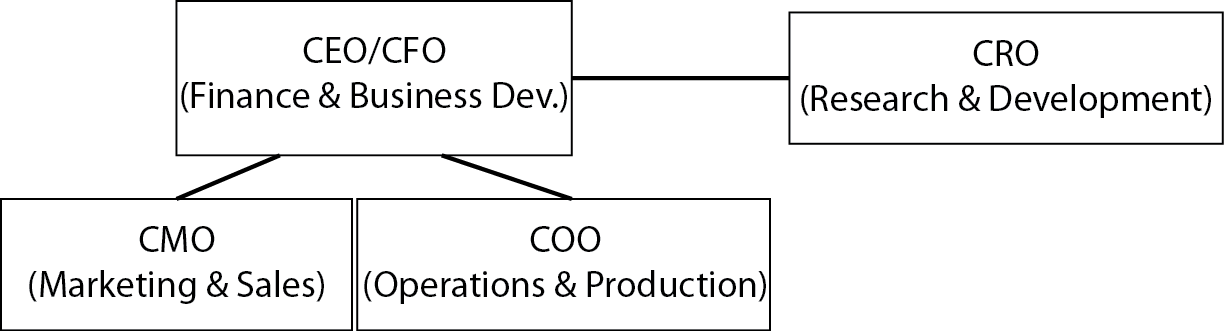
\includegraphics[width=5.5in]{./pngs/organizational-model.png}
\end{center}
\caption{The H2O IQ corporation's corporate model values R\&D highly.}
\label{fig:structure}
\end{figure}

\section{Competitive Landscape}

Current products on the market that have similar goals to H2O IQ include the Koubachi system and Hydrospikes.

The Koubachi system is designed to ``give your plant a voice''.  It has an array of sensors which are available to be read on a website and compared to established plant care models.  It does not have actuation as the H2O IQ, so while it has additional sensors it cannot help you care for your plant when you are away.  The Koubachi system retails for EUR119.00, approximately USD150, which is significantly more than H2O IQ is projected to retail for.

Hydrospikes are ``worry-free automatic watering kits''.  They are simple plastic spikes that can be filled with water and inserted into soil next to plants to water them gradually over several days.  This product, however, does not have sensors or internet connectivity, and thus it is in a very different price bracket, costing USD9 for three units.

\section{Model Spreadsheets}
See Table \ref{tab:profit}

%\begin{figure}[h]
%\begin{center}
%\includegraphics[scale=0.36]{./pngs/XXX.png}
%\end{center}
%\caption{YYY}
%\label{fig:XXX}
%\end{figure}

%\begin{table}
\begin{sidewaystable}
\begin{tabular}{l||r|r|r|r|r}
&2012&2013&2014&2015&2016\\
 \hline 
Sales Price &0&\$99.99 &\$99.99 &\$99.99 &\$99.99 \\
\# Units Sold &0&1000&16000&38000&36000\\
\hline
Net Sales &0&\$99,990.00 &\$1,599,840.00 &\$3,799,620.00 &\$3,599,640.00 \\
\hline 
Cumulative Net Sales &0&\$99,990.00 &\$1,699,830.00 &\$5,499,450.00 &\$9,099,090.00 \\
\hline
Material Costs by Unit (2 stakes + server)&  &  &  &  &\\
~~ Moisture Sensor &  &0.02&0.02&0.02&0.02\\
~~ Servo &  &1&0.95&0.9&0.9\\
~~ PCB &  &0.5&0.3&0.2&0.2\\
~~ Wireless Radio &  &1.5&1.2&1&0.9\\
~~ Micro-controller &  &0.3&0.25&0.23&0.2\\
~~ Solar Cell &  &1&0.96&0.93&0.92\\
~~ PCB components &  &0.05&0.04&0.03&0.03\\
~~ Plastic Enclosure &&0.1&0.1&0.1&0.1\\
~~ Server &  &20 &17&16&16\\
~~~~ Total Unit Material Costs &0&\$28.94 &\$24.64 &\$22.82 &\$22.54 \\
Labor By Unit &  &6&6&6&6\\
~~~~ Total Unit Costs &0& 34.94&30.64&28.82&28.54\\
~~~~ Total Stake Cost&0&4.47&3.82&3.41&3.27\\
\hline 
Cost of Products Sold &0&\$34,940&\$490,240&\$1,095,160&\$1,027,440\\
Gross Margin &0&\$65,050 &\$1,109,600 &\$2,704,460 &\$2,572,200 \\
\% Gross Margin &0&65.10\%& 69.36\% & 71.18\% &71.46\%\\
\hline
Development Costs&\$13,462&\$150,000& \$100,000&\$100,000&\$100,000\\
Tooling Costs &0&\$158,872&0&0&0\\
Overhead Costs &0&\$30,000&\$40,000&\$40,000&\$40,000\\
Marketing (@ 13\% Net Sales) &0&\$12,998.70 &\$207,979.20 &\$493,950.60 &\$467,953.20 \\
Other (@ 8\%) &0&\$7,999.20 &\$127,987.20 &\$303,969.60 &\$287,971.20 \\
\hline 
Total Operating Expenses &\$13,461.54 &\$394,809.90 &\$966,206.40 &\$2,033,080.20 &\$1,923,364.40 \\
\hline 
Pre-Tax Profit &(\$13,461.54)&(\$294,819.90)&\$633,633.60 &\$1,766,539.80 &\$1,676,275.60 \\
\% Profit &N/A&-294.85\%&39.61\%&46.49\%&46.57\%\\
\hline 
Cumulative Profit &(\$13,461.54)&(\$308,281.44)&\$325,352.16 &\$2,091,891.96 &\$3,768,167.56 \\
\end{tabular}
\caption{\label{tab:profit}Most Likely Profit Scenario}
\end{sidewaystable}


\bibliographystyle{plain}
\bibliography{businessplan}
\end{document}
